\documentclass[11pt]{beamer}
\usepackage[utf8]{inputenc}
\usepackage[T1]{fontenc}
\usepackage{lmodern}
\usepackage[english]{babel}
\usepackage{booktabs}
\usepackage{fontawesome}
\usetheme{Darmstadt}
\setbeamertemplate{navigation symbols}{}
\setbeamertemplate{footline}{
	\begin{beamercolorbox}[ht=3ex,leftskip=1.4cm,rightskip=.3cm]{author in head/foot}
		\hfill \insertframenumber
		\vspace*{0.07cm}
	\end{beamercolorbox}
} 
\usepackage{url}
\usepackage{hyperref}

% color def
\usepackage{color}
\definecolor{darkred}{rgb}{0.6,0.0,0.0}
\definecolor{darkgreen}{rgb}{0,0.50,0}
\definecolor{lightblue}{rgb}{0.0,0.42,0.91}
\definecolor{orange}{rgb}{0.99,0.48,0.13}
\definecolor{grass}{rgb}{0.18,0.80,0.18}
\definecolor{pink}{rgb}{0.97,0.15,0.45}

\usepackage{listings}
\usepackage{upquote}


\newcommand\Wider[2][3em]{%
\makebox[\linewidth][c]{%
  \begin{minipage}{\dimexpr\textwidth+#1\relax}
  \raggedright#2
  \end{minipage}%
  }%
}

\lstdefinestyle{Python}{
    language=Python,
    morekeywords=[1]{,as,assert,nonlocal,with,yield,self,True,False,None,} % Python builtin
	morekeywords=[2]{,__init__,__add__,__mul__,__div__,__sub__,__call__,__getitem__,__setitem__,__eq__,__ne__,__nonzero__,__rmul__,__radd__,__repr__,__str__,__get__,__truediv__,__pow__,__name__,__future__,__all__,}, % magic methods
	morekeywords=[3]{,object,type,isinstance,copy,deepcopy,zip,enumerate,reversed,list,set,len,dict,tuple,range,xrange,execfile,real,imag,reduce,str,repr,}, % common functions
	morekeywords=[4]{,Exception,NameError,IndexError,SyntaxError,TypeError,ValueError,OverflowError,ZeroDivisionError,}, % errors
	morekeywords=[5]{,ode,fsolve,sqrt,exp,sin,cos,arctan,arctan2,arccos,pi, array,norm,solve,dot,arange,isscalar,max,sum,flatten,shape,reshape,find,any,all,abs,plot,linspace,legend,quad,polyval,polyfit,hstack,concatenate,vstack,column_stack,empty,zeros,ones,rand,vander,grid,pcolor,eig,eigs,eigvals,svd,qr,tan,det,logspace,roll,min,mean,cumsum,cumprod,diff,vectorize,lstsq,cla,eye,xlabel,ylabel,squeeze,}, % numpy / math
	%morestring=*[b]{"},
    basicstyle=\ttfamily,
   	backgroundcolor=\color{white},
   	commentstyle=\color{darkgreen}\slshape,
   	keywordstyle=\color{blue}\bfseries\itshape,
   	keywordstyle=[2]\color{blue}\bfseries,
   	keywordstyle=[3]\color{grass},
   	keywordstyle=[4]\color{red},
   	keywordstyle=[5]\color{orange},
   	stringstyle=\color{darkred},
   	emphstyle=\color{pink}\underbar,
    % honek neretako bakarrik die
    %deletekeywords=[2]{next,set},
    %deletekeywords=[3]{next,set},
}

% General Setting of listings
\lstset{
    style=Python,
	tabsize=4,
	aboveskip=1em,
	breaklines=true,
	abovecaptionskip=-6pt,
	captionpos=b,
	escapeinside={\%*}{*)},
	frame=single,
	numbers=left,
	numbersep=8pt,
	numberstyle=\tiny,
    showstringspaces=false,
}

\definecolor{delim}{RGB}{20,105,176}
\definecolor{numb}{RGB}{106, 109, 32}
\definecolor{string}{rgb}{0.64,0.08,0.08}

\lstdefinelanguage{json}{
    showspaces=false,
    showtabs=false,
    breaklines=true,
    postbreak=\raisebox{0ex}[0ex][0ex]{\ensuremath{\color{gray}\hookrightarrow\space}},
    breakatwhitespace=true,
    basicstyle=\ttfamily\small,
    upquote=true,
    morestring=[b]",
    stringstyle=\color{string},
    literate=
     *{0}{{{\color{numb}0}}}{1}
      {1}{{{\color{numb}1}}}{1}
      {2}{{{\color{numb}2}}}{1}
      {3}{{{\color{numb}3}}}{1}
      {4}{{{\color{numb}4}}}{1}
      {5}{{{\color{numb}5}}}{1}
      {6}{{{\color{numb}6}}}{1}
      {7}{{{\color{numb}7}}}{1}
      {8}{{{\color{numb}8}}}{1}
      {9}{{{\color{numb}9}}}{1}
      {\{}{{{\color{delim}{\{}}}}{1}
      {\}}{{{\color{delim}{\}}}}}{1}
      {[}{{{\color{delim}{[}}}}{1}
      {]}{{{\color{delim}{]}}}}{1},
}

\usepackage{tikz}
\usetikzlibrary{calc,shapes.multipart,chains,arrows,positioning}
\usetikzlibrary {shapes.misc} 
\usetikzlibrary{shadows.blur}
\usetikzlibrary{matrix}
\tikzset{
stack_item/.style={rounded rectangle, rounded rectangle arc length=90,draw, anchor=center, fill=white, minimum width=2cm, minimum height=0.7cm},
bar/.style={rounded rectangle, minimum width=3cm, fill=black, blur shadow={shadow blur steps=5,shadow blur extra rounding=1.3pt}},
message/.style={rectangle, fill=white, color=white, text=black},
bowling_pin/.style={circle, draw, line width=0.6mm, color=red, text=black, minimum width=8mm},
empty/.style={circle, draw, line width=0.6mm, color=white, text=black, minimum width=8mm},
table_cell/.style={rectangle, draw, color=black, text=black, minimum size=12mm}
}

\tikzset{
	squarecross/.style={
		draw, rectangle,minimum size=18pt, fill=orange!80,
		inner sep=0pt, text=black,
		path picture = {
			\draw[-,black]
			(path picture bounding box.north west) --
			(path picture bounding box.south east)
			(path picture bounding box.south west) --
			(path picture bounding box.north east);
		}
	},
	list/.style={
		very thick, rectangle split,
		rectangle split parts=2, draw,
		rectangle split horizontal, minimum size=18pt,
		inner sep=4pt, text=black,
		rectangle split part fill={red!20, blue!20}
	},
	->, start chain, very thick,
	chain_arrow/.style={*->, thick}
}

\usetikzlibrary{arrows.meta}
\tikzset{
    queue element/.style={
        draw,very thin,rounded corners,
        fill=white,
        minimum width=1cm,minimum height=.5cm,
        font=\sffamily\footnotesize
    },
    priority element/.style={
            draw,very thin,rounded corners,
            fill=white,
            minimum width=1cm,minimum height=1cm,
            text width=0.75cm,align=center,
            font=\sffamily\footnotesize
        },
    >={[scale=0.8]Triangle}
}

\author{Data Structures}
\title{\huge{Extending the Queue}}
\titlegraphic{
\includegraphics[width=3cm]{img/UPNA}}
\date[]{2024-2025}
\subject{Data Structures}
%\subtitle{}
%\logo{}
%\institute{}
%\date{}
%\subject{}
%\setbeamercovered{transparent}
%\setbeamertemplate{navigation symbols}{}

\AtBeginSection[]{
	\begin{frame}[plain]
		\frametitle{}
		\tableofcontents[currentsection, hideothersubsections]
	\end{frame}
}

\begin{document}
\begin{frame}[plain]
	\maketitle
\end{frame}

\begin{frame}
	\tableofcontents
\end{frame}

\section{Double-Ended Queue}

\begin{frame}\frametitle{What is a Double Queue}
\begin{itemize}
\item A double-ended queue, also known as a Deque, is a generalization to a queue
    \begin{itemize}
    \item Elements can be added or removed from the front or back
    \item It is pronounced as \textit{deck}
    \item In some cases it can be found as dequeue
    \end{itemize}
\item Sometimes restrictions are added to how items are inserted or removed
    \begin{itemize}
    \item What would happen if we prohibit adding or removing elements just from one side?
    \end{itemize}
\end{itemize}
\end{frame}

\begin{frame}\frametitle{Operations on a Deque}
\begin{center}
\scalebox{1}{
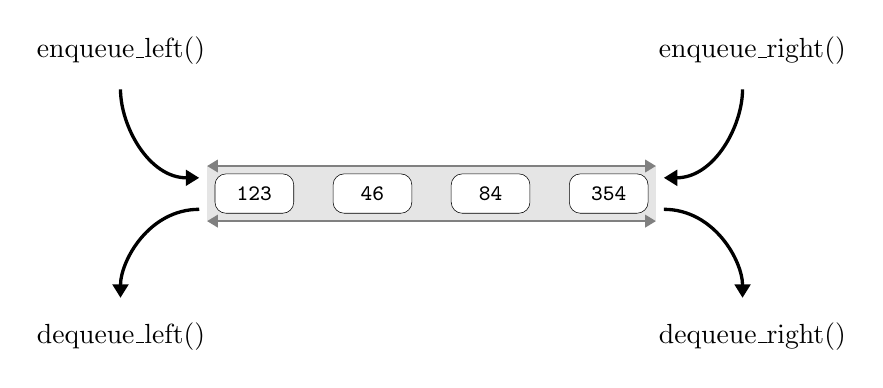
\begin{tikzpicture}
\fill[gray!20] (5.1,.35) rectangle (-.6,-.35);
\draw[gray,thick,<->] (-.6,.35) -- (5.1,.35);
\draw[gray,thick,<->] (-.6,-.35) -- (5.1,-.35);
\foreach \i/\name in {0/123,1/46,2/84,3/354}
    \node[queue element] (elem_\i) at (1.5*\i,0) {\texttt{\name}};
\draw[->,very thick, shorten >=5pt] (5.2,-0.2) to[out=0,in=90] (6.2,-1.5) node[below right=0 and -1.2] {dequeue\_right()};
\draw[<-,very thick, shorten >=5pt] (5.2,0.2) to[out=0,in=270] (6.2,1.5) node[above right=0 and -1.2] {enqueue\_right()};
\draw[->,very thick, shorten >=5pt] (-0.7,-0.2) to[out=180,in=90] (-1.7,-1.5) node[below right=0 and -1.2] {dequeue\_left()};
\draw[<-,very thick, shorten >=5pt] (-0.7,0.2) to[out=180,in=270] (-1.7,1.5) node[above right=0 and -1.2] {enqueue\_left()};
\end{tikzpicture}
}
\end{center}
\end{frame}

\begin{frame}[fragile]\frametitle{Implemented on Python}
\begin{itemize}
\item Python contains a module for more specialized collection structures
    \begin{itemize}
    \item \href{https://docs.python.org/3/library/collections.html}{\color{blue}\underline{collections}}
    \end{itemize}
\item An implementation of a Deque is included
    \begin{itemize}
    \item Implemented using linked lists
    \end{itemize}
\end{itemize}
\begin{lstlisting}
import collections

d = collections.deque()
d.append('b')
d.appendleft('a')
d.popleft()
d.pop()
\end{lstlisting}
\end{frame}


\section{Priority Queue}

\begin{frame}\frametitle{Priority Queue}
\begin{itemize}
\item Sometimes an element on a queue has a higher priority than the others
    \begin{itemize}
    \item This means that the elements should be dequeued before the others
    \item Queues at an amusement park
    \item Boarding an airplane
    \end{itemize}
\item Each time an item is enqueued \textbf{we give it a priority}
\item To dequeue an item we dequeue the oldest element inserted with the lowest priority
\end{itemize}
\end{frame}

\subsection{Two Approaches}

\begin{frame}\frametitle{Sorted Insertion I}
\begin{center}
\scalebox{1}{
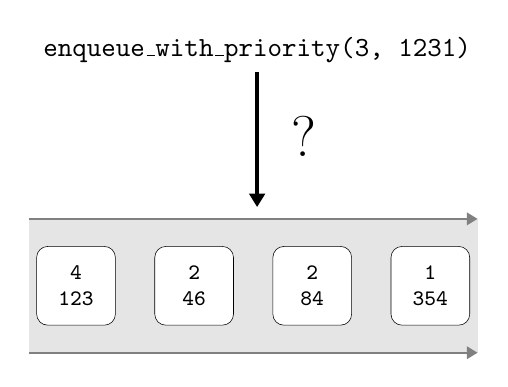
\begin{tikzpicture}
\fill[gray!20] (5.1,.85) rectangle (-.6,-.85);
\draw[gray,thick,->] (-.6,.85) -- (5.1,.85);
\draw[gray,thick,->] (-.6,-.85) -- (5.1,-.85);
\foreach \i/\name/\pri in {0/123/4,1/46/2,2/84/2,3/354/1}
    \node[priority element] (elem_\i) at (1.5*\i,0) {\texttt{\pri}\\\texttt{\name}};
\node (text) at (2.3, 3) {\texttt{enqueue\_with\_priority(3, 1231)}};
\draw[->, very thick] (text) -- (2.3, 1) node[above right=0.5 and  0.3] {\huge ?};

%\draw[draw=none] (0,1) to[out=180,in=90] (0,1) node[above right=2 and -1] {\texttt{enqueue\_with\_priority(3, 1231)}};
\end{tikzpicture}
}
\end{center}
\end{frame}


\begin{frame}\frametitle{Sorted Insertion II}
\begin{block}{}
Each time an element is enqueued we will insert it in its appropriate location according to the given priority. \\When dequeueing we follow the normal queue procedure.
\end{block}
\vspace{0.4cm}
\begin{center}
\scalebox{1}{
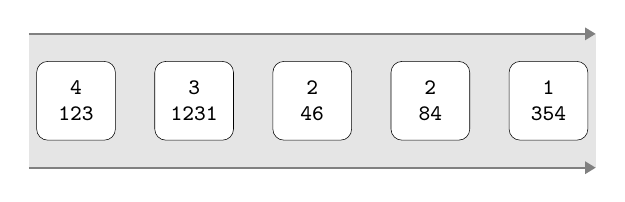
\begin{tikzpicture}
\fill[gray!20] (6.6,.85) rectangle (-.6,-.85);
\draw[gray,thick,->] (-.6,.85) -- (6.6,.85);
\draw[gray,thick,->] (-.6,-.85) -- (6.6,-.85);
\foreach \i/\name/\pri in {0/123/4,1/1231/3,2/46/2,3/84/2,4/354/1}
    \node[priority element] (elem_\i) at (1.5*\i,0) {\texttt{\pri}\\\texttt{\name}};
\end{tikzpicture}
}
\end{center}
\end{frame}


\begin{frame}\frametitle{Search on Extraction I}
\begin{center}
\scalebox{1}{
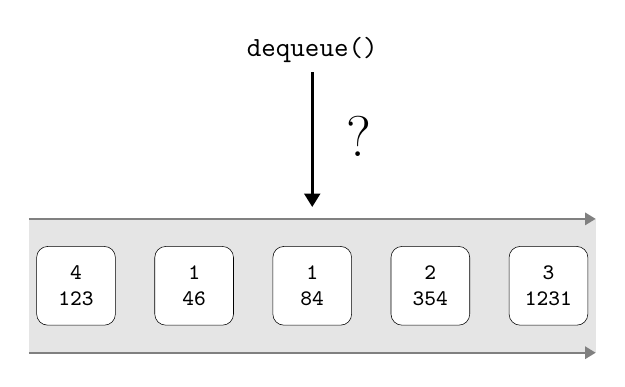
\begin{tikzpicture}
\fill[gray!20] (6.6,.85) rectangle (-.6,-.85);
\draw[gray,thick,->] (-.6,.85) -- (6.6,.85);
\draw[gray,thick,->] (-.6,-.85) -- (6.6,-.85);
\foreach \i/\name/\pri in {0/123/4,1/46/1,2/84/1,3/354/2,4/1231/3}
    \node[priority element] (elem_\i) at (1.5*\i,0) {\texttt{\pri}\\\texttt{\name}};
\node (text) at (3, 3) {\texttt{dequeue()}};
\draw[->, very thick] (text) -- (3, 1) node[above right=0.5 and  0.3] {\huge ?};
\end{tikzpicture}
}
\end{center}
\end{frame}


\begin{frame}\frametitle{Search on Extraction II}
\begin{block}{}
The elements are inserted as in a normal queue. \\
When dequeueing the first element from the front that has the lowest priority will be extracted.
\end{block}
\vspace{0.4cm}
\begin{center}
\scalebox{1}{
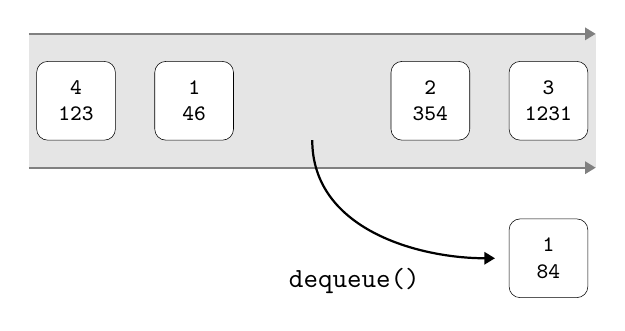
\begin{tikzpicture}
\fill[gray!20] (6.6,.85) rectangle (-.6,-.85);
\draw[gray,thick,->] (-.6,.85) -- (6.6,.85);
\draw[gray,thick,->] (-.6,-.85) -- (6.6,-.85);
\foreach \i/\name/\pri in {0/123/4,1/46/1,3/354/2,4/1231/3}
    \node[priority element] (elem_\i) at (1.5*\i,0) {\texttt{\pri}\\\texttt{\name}};

\node[priority element] (extracted) at (6, -2) {\texttt{1}\\\texttt{84}};
\draw[->, thick, shorten >=5pt] (3,-0.5) to[out=-90, in=180] (extracted.west) node[below left=0 and  1] {\texttt{dequeue()}};
%\draw[<-,very thick, shorten >=5pt] (-0.7,0.2) to[out=180,in=270] (-1.7,1.5) node[above right=0 and -1.2] {enqueue\_left()};
\end{tikzpicture}
}
\end{center}
\end{frame}


\section{Circular Buffer}

\begin{frame}\frametitle{Circular Buffer}
\begin{itemize}
\item We can limit the size of a queue
    \begin{itemize}
    \item As new elements are inserted in the queue, old ones are removed
    \end{itemize}
\item In some cases we are only interested in the latest data
    \begin{itemize}
    \item Streaming video/audio
    \item Buffering data streams, hence the name
    \end{itemize}
\item Follows FIFO
\item There is no beginning or end to the buffer, only for the data it stores
\end{itemize}
\end{frame}

\begin{frame}\frametitle{Using a Circular Buffer}
\begin{center}
\scalebox{1.5}{
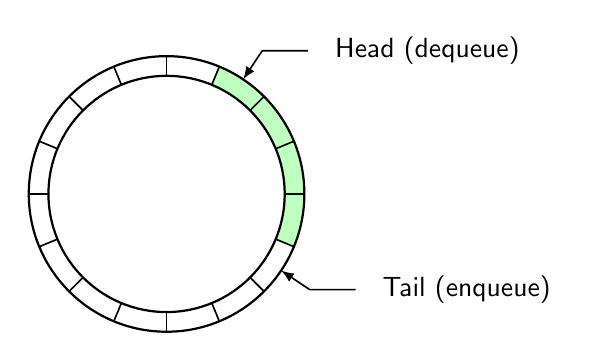
\begin{tikzpicture}[>=latex,font=\sffamily,semithick,scale=1.75]
    \fill [green!25] (0,0) -- (67.5:1) arc [end angle=-22.5, start angle=67.5, radius=1] -- cycle;
    \draw [thick] (0,0) circle (1);
    \foreach \angle in {90,67.5,...,-67.5}
        \draw[-] (\angle:1) -- (\angle-180:1);
    \node [circle,thick,fill=white,draw=black,align=center,minimum size=3cm] at (0,0) {};
    \draw [<-] (56.25:1) -- (56.25:1.25) -- +(.333,0)
        node [right,inner xsep=.333cm] (Head) {Head (dequeue)};
    \draw [<-] (-33.75:1) -- (-33.75:1.25) -- +(.333,0)
        node [right,inner xsep=.333cm] (Tail) {Tail (enqueue)};
\end{tikzpicture}
}
\end{center}
\end{frame}

\begin{frame}\frametitle{Exercise}
\begin{block}{}
\Huge\centering Create a circular buffer by using a size limited queue.
\end{block}
\begin{itemize}
\item What happens if we insert when the queue is full?
\item How can we make sure that we always dequeue the oldest element?
\end{itemize}
\end{frame}


\begin{frame}\frametitle{Improving a Circular Buffer}
\begin{center}
\scalebox{2}{
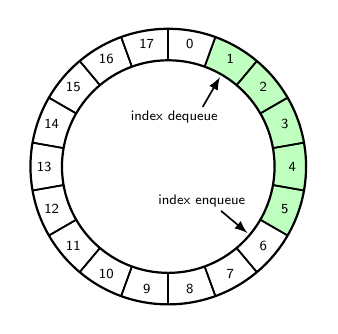
\begin{tikzpicture}[>=latex,font=\sffamily,semithick,scale=1.75]
    \fill [green!25] (0,0) -- (70:1) arc [end angle=-30, start angle=70, radius=1] -- cycle;
    \draw [thick] (0,0) circle (1);
    \foreach \angle in {0,1,...,17}
        \draw[-] (\angle*20-90:1) -- (\angle*20-180-90:1);
    \foreach \angle in {0,1,...,17}
        \draw[draw=none] (80-\angle*20:1) -- (80-\angle*20:0.9) node {\tiny\angle};
    \node [circle,thick,fill=white,draw=black,align=center,minimum size=2.7cm] at (0,0) {};
    \draw[->] (60:0.5) -- (60:0.75) node [below left=0.3 and -0.1] {\tiny index dequeue};
    \draw[->] (-40:0.5) -- (-40:0.75) node [above left=0.2 and -0.1] {\tiny index enqueue};
\end{tikzpicture}
}
\end{center}
\end{frame}


\begin{frame}\frametitle{Exercise}
\begin{block}{}
\Huge\centering Create a circular buffer by using a size limited queue. Use indexes to access the elements.
\end{block}
\begin{itemize}
\item How do we handle the indices?
\item What happens if one goes over the size limit?
\end{itemize}
\end{frame}

\end{document}